

%\section{Design Method}\label{sec:design_method}
This chapter focusses on each of the code generation phases and what our contributions are to this compiler. This chapter describes how a compiler without support for explicit datapaths (which is described in Section \ref{sec:basic_compiler_design}) is maintained and extended to a compiler with support for explicit datapaths. 

%Discuss maintaining, process of porting from llvm3.8 to LLVM4.0, and discuss new version LLVM5.0. Mention that this upgrade to 4.0 also drastically improved vectorization because the community develops this constantly. (maybe add example of CNN)

%TODO: move vectorization to here? Noooo.

\section{Back-end Code Generation}\label{sec:code_generation}
This section briefly discusses each of the code generation stages, which includes custom passes and standard passes supplied by the LLVM framework. Before generating code, it uses LLVM's front-end to translate a high-level language to an intermediate representation, called LLVM-IR which can be further optimized and used as input for our back-end. The code generation passes in the back-end specific compiler can be categorized in three major categories.
%include an image with the pipeline having all these components.

%TODO: refere to problem where instr have no common operand, so it seems unrelated. 

%TODO: add text that explains the color, instruction selection is copied mostly from another architectures, and was already updated according to our architecture. / Hazard recognizer has partially been copied from other architectures, but was not suitable and has, therefore, been modified and tested. / Delay slot is a custom pass that was already implemented, but we have modified it to be more efficient. / Packetizer pass is as delivered, with a minor modification with hardly any efford.  / Bypass Regs is a custom pass that we developed during the duration of our work.

Firstly, the top row in Figure \ref{fig:simd_backend} shows passes that work on creating a schedule. The second row illustrates a sequence of compilation passes that do back-end specific transformations. Here special features that our architecture has are taken care of. At last, with an LLVM internal representation of back-end specific code for the target architecture, it emits assembly or ELF object code (depicted in the rightmost part of the image) that the processor can understand.

\begin{figure}[H]
\centering
\hspace*{-.12in}
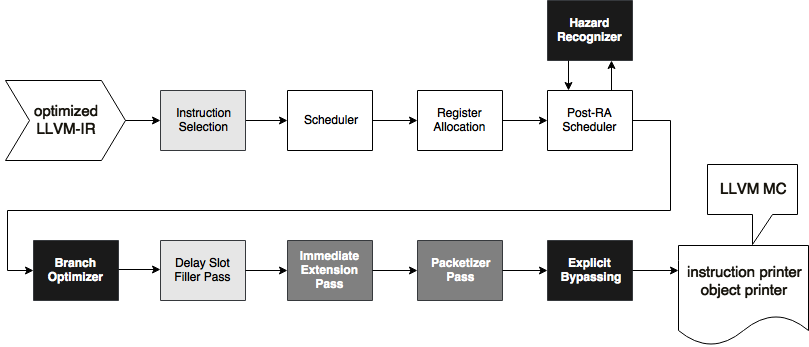
\includegraphics[width=\textwidth]{figures/code_generation}
%TODO: change orange to yellow and yellow to orange in picture. 
\caption{Overview of the phases that the back-end is comprised of.}
\label{fig:simd_backend}
\end{figure}

Note that the passes are marked from light to dark, where a black background means that the pass was created during this project and are the main contributions of this work. Dark grey indicates that a pass is extended or improved, light grey indicates the pass has hardly changed and a white background means that the pass is supplied by LLVM.

%A list of all components that follow in the following section.
\begin{itemize}
	\item \textbf{Instruction Selection:} Uses a DAG, called \texttt{SelectionDAGs}, an abstraction for code representation suitable for phases ranging from instruction selection, legalization to lowering. Instruction selection is implemented in  \texttt{SimdISelDAGToDAG}, which is derived from \texttt{SelectionDAGISel} and consists of a bunch of transformations to transform specific instructions into instruction that are supported by our architecture. For example, transforming operations on immediate values with a value higher than one byte is partially implemented here. Lowering nodes of a DAG is done in \texttt{SimdISelLowering}, which is derived from \texttt{TargetLowering}. There the SIMD intrinsics and ISD instructions are lowered to \emph{Machine Instructions} (MI) and sequences of MIs.
%\item \textbf{Scheduling:} Transforms a directed acyclic graph into an ordered list of instructions.
%\item \textbf{Register allocation:} Assigns physical registers to virtual registers of a list of instructions in SSA form.
	\item \textbf{Instruction Scheduler:} MIScheduler supplied by LLVM\\
MIScheduler is an instruction scheduler which supports VLIW scheduling. Considering there are two issue slots in this architecture, a VLIW scheduler would meet our requirements very well. One and two schedulers are defined for four-stage pipeline and five-stage pipeline respectively. The four-stage pipeline scheduler is the default one while the five-stage pipeline has the default one, and an additional post-register allocation scheduler.
	\item \textbf{Register Allocation:} Greedy Allocator supplied by LLVM\\
	The Greedy allocator is a default allocator in LLVM. Since there is no specific requirement to register allocation, for now, the default allocator is suitable. Apart from the default register allocator, there are more register allocators to choose from and, it is possible to implement a custom register allocator.
	\item \textbf{Post-Register Allocation Scheduler:} A second scheduling pass which is only needed when generating code for a five-stage pipeline configuration, and is disabled otherwise. The post-RA scheduler uses a hazard recognizer which decides whether to prefer certain instruction over other instructions to detect and resolve RaW hazards.
	\item \textbf{Hazard Recognizer:} Consecutive instructions may have hazards with the five-stage pipeline configured. That is when an instruction uses an operand defined in the previous cycle but has a latency of two cycles. For this thesis, we have implemented LLVM's \texttt{ScoreboardHazardRecognizer} to detect and resolve these hazards.
	\item \textbf{Branch Optimizer:} An inefficiency in the generated code was observed where two jump operations control the work flow, but one jump is not necessary when it jumps to the successor that follows immediately. 
	%TODO: check implements / extends / derived
	\item \textbf{Delay Slot Filler:} For this architecture, jump and branch instructions modify the program counter (PC) during the instruction decode stage. At that point, the instruction that follows the jump has already been fetched. The slot that follows a jump or branch instruction is called a delay slot. This pass aims to utilize delay slots by filling them with useful instructions.% that come after a jump or conditional branch instruction, i.e. instructions that modify the program counter.%VERIFY: `or e.g.?
	\item \textbf{Immediate Extension:} In principle, immediate operations have a one-byte immediate operand. However, sometimes you may want to use a larger immediate. This pass allows us to use a larger immediate operand using \texttt{zimm} and \texttt{simm} instruction. These instructions have an 18-bit operand that allows for larger constants to be used.% will be a prefix of the original 8 bits  or using a shift to put a value in a register (up to 32 bits).
	\item \textbf{Packetizer:} This pass creates VLIW bundles that consist of a scalar and a vector instruction, by consulting whether an issue slot is available on which the operation can execute. This pass implements VLIW packetizer supplied by the LLVM framework.
	\item \textbf{Explicit Bypassing:} This pass exploits explicit datapaths in the generated code by using the bypass network. This is developed as a post-processing pass, but can be replaced by any of the approaches discussed in Chapter \ref{sec:expl_bp_impl}.
	\item \textbf{Instruction Printer:} MC is a sub-project of LLVM, which uses \texttt{MCInst} to represent an instruction which is different from the code generators notion of a \texttt{MachineInstr}. MC is used during the last code generation stage when printing the instructions to a given output format. Printing for different output formats is further divided in binary format and SIMD assembly language in XAS-format. 
\end{itemize}

\begin{table}[t!]
\caption{Relations between architecture design features and code generation phases.}
\begin{center}
\begin{tabular}{@{}l l l@{}}
\toprule
\textbf{Feature} & \textbf{Code Gen. Pass} & \textbf{Explanation}\\ \hline
Hardware Pipeline 	& Delay Slot Filler 		& This pass utilizes the delay slots (which is\\
				&					& a product lockstep pipelining).\\
			 	& Hazard Recognizer 	& This pass is necessary for a five-stage \\
				&					& pipeline configuration where not all\\
				&					& instructions have a single cycle latency.\\
Bit-width 			& Immediate Extension 	& Lowering immediate operands is done\\
				&				    	& differently for different data bit-width. \\
ISA extension		& Instruction Selection 	& New instructions need to be described in\\
				& \& Instruction Lowering	& the back-end. \\
Explicit datapaths 	& Explicit Bypassing		& This optional pass is developed to exploit\\
				&					& explicit datapaths. It can be enabled\\
				&					& using compiler flag \texttt{-explicit}. \\
\bottomrule
\end{tabular}
\end{center}
\label{table:rel_feature_pass}
\end{table}%

The following sections give a more elaborate discussion on each custom pass and describe their relation to each other. However, before that have a look at Table \ref{table:rel_feature_pass} which gives an overview of the passes responsible for each of the features from Chapter \ref{sec:problem_statement}. 

%TODO: validate and update
\section{Custom Passes}
This section describes the custom passes in more detail. Dependencies and relations to other passes are described. Furthermore, it will discuss the entire toolchain, which includes an assembler, a linker, and a simulator. 

\subsection{Hazard Recognizer}\label{sec:hazard_recogn}
When generating code for a four-stage pipeline configuration, all instructions have a latency of one cycle. In that case, hazard recognition is not necessary.
In order to support code generation for a five-stage pipeline, a hazard recognizer has been developed. The hazard recognizer is used by the post-RA scheduler to determine whether two consecutive instructions can be scheduled after each other. 

\lstset{style=customasm}
\begin{lstlisting}
addi r13, r0, 14
addi r12, r0, 10
mul  r2,  r5, r13  # latency=2
mul  <@\hspace{1px}\textcolor{red!70!black}{r3}\hspace{1px}@>,  r6, r12  # latency=2
add  r2,  r2, <@\hspace{1px}\textcolor{red!70!black}{r3}\hspace{1px}@>   # RaW dependency
\end{lstlisting}

It detects hazards by considering whether an operation has a RaW dependency with instruction that came prior to it. A true hazard is when the instruction that came prior to it has a RaW dependency and a latency of more than one cycle. The \emph{post-register allocation} (Post-RA) scheduler does a linear scan through the list of operation and queries the hazard recognizer whether an instruction can be scheduled. When it detects a hazard, it will consider other instructions that are ready to be scheduled, and if there are none available without a hazard, it will insert a no-op and the processor will be stalled for a cycle.

%It recognizes hazards by looking at whether the current instruction to be scheduled uses a register that is defined by the instruction issued in the previous cycle, which also has a latency of more than one cycle. If this is the case, we have a hazard and the instruction under consideration can not be scheduled in the current cycle. At this point we will consider other instructions that are ready to be scheduled and if there are none available without hazards, we will insert a no-op.

\subsection{Branch Optimizer}
%WORKING RIGHT HERE. ADD EXAMPLE CASES FROM BRANCH OPT.
There were many double branch instructions in loop structures. Preliminary benchmarks already showed that a double branch instruction does not always help. For example, consider the assembly code fragments in Listing \ref{lst:br_opt_1} and Listing \ref{lst:br_opt_2}. Note that at this point, the delay slots that always follow after a jump or branch instruction are still absent because the delay slot filler pass has not run yet.

\captionof{lstlisting}{Fragment of assembly code to illustrate the first and second cases that are considered by the branch optimization pass.}\label{lst:br_opt_1}
\begin{center}
\hspace{2px}\begin{minipage}{.475\textwidth}
\begin{lstlisting}[frame=tlrb]
$BB1:
    addi   r1, r1, 1
    sfltsi r1, 64
    <@\hspace{1px}\textcolor{red!70!black}{bf}\hspace{1px}@>     <@\hspace{1px}\textcolor{red!70!black}{\$BB1}\hspace{1px}@>
    <@\hspace{1px}\textcolor{red!70!black}{j}\hspace{1px}@>      <@\hspace{1px}\textcolor{red!70!black}{\$BB2}\hspace{1px}@>
$BB2:      <@ $\hdots$@>
\end{lstlisting}
\end{minipage}\hfill
\begin{minipage}{.475\textwidth}
\begin{lstlisting}[frame=tlrb]
$BB1:
    addi   r1, r1, 1
    sfltsi r1, 64
    <@\hspace{1px}\textcolor{red!70!black}{bf}\hspace{1px}@>     <@\hspace{1px}\textcolor{red!70!black}{\$BB1}\hspace{1px}@>
$BB2:      <@ $\hdots$@>
           <@ $\hdots$@>
\end{lstlisting}
%\vspace{1.9em}
\end{minipage}
\end{center}

\begin{enumerate}
  \item The first case is where a block ends with a jump instruction to the block that immediately follows. The example shows a loop in which a counter is incremented until it reaches sixty-four. As long as the counter is less than that, the flag will be true and the branch is executed. When the counter increases, at some point the condition breaks and the flag becomes false. The program counter then points to the first instruction after the branch instruction, which is a jump instruction. However, the jump goes to the successor that immediately follows. When the jump is removed, the first instruction after the branch instruction is still the successor block that immediately follows. Hence the behaviour without that jump is identical and the superfluous jump can be removed.
  \item The second case has a branch instruction to the block that immediately follows and a jump to somewhere else. The first step then is to reverse the branch condition. This can be achieved by changing a \texttt{bf} (branch flag) instruction into a \texttt{bnf} (branch not flag) and vice versa. After the branch is reversed, the situation becomes a jump instruction to the block that immediately follows and a branch instruction to somewhere else. 
\end{enumerate}

\captionof{lstlisting}{Fragment of assembly code to illustrate the third case that is covered by the branch optimization pass.}\label{lst:br_opt_2}
\begin{center}
\hspace{2px}\begin{minipage}{.475\textwidth}
\begin{lstlisting}[frame=tlrb]
$BB2: <@$\hdots$@>
    sf condition  # set-flag
    <@\hspace{1px}\textcolor{red!70!black}{bf}\hspace{1px}@> <@\hspace{1px}\textcolor{red!70!black}{\$BB3}\hspace{1px}@>
    <@\hspace{1px}\textcolor{red!70!black}{j}\hspace{1px}@>  <@\hspace{1px}\textcolor{red!70!black}{\$BB2}\hspace{1px}@>
$BB3: <@$\hdots$@>
\end{lstlisting}
\end{minipage}\hfill
\begin{minipage}{.475\textwidth}
\begin{lstlisting}[frame=tlrb]
$BB2: <@$\hdots$@>
    sf  condition  # set-flag
    <@\hspace{1px}\textcolor{red!70!black}{bnf}\hspace{1px}@> <@\hspace{1px}\textcolor{red!70!black}{\$BB2}\hspace{1px}@>
$BB3: <@$\hdots$@>
     <@ $\hdots$@>
\end{lstlisting}
%\vspace{1.9em}
\end{minipage}
\end{center}

When a (double) jump intruction(s) jumps to a successor that immediately follows, the branch optimizer can always remove one jump with these cases.



%END BRANCH OPT DESCRIPTION

\subsection{Delay Slot Filler}
During the execution of a conditional branch or jump instruction the \emph{program counter} (PC) is modified while the instruction is in the \emph{instruction decode} (ID) stage. A side product of lockstep pipelining which is introduced in Chapter \ref{sec:datapaths}, is that when a jump instruction is being decoded in the ID stage, the next instruction with $PC = PC+4$ has already been fetched from IMEM before the jump is executed. Therefore, the instruction that is followed by the jump instruction is executed presumptuously, which is referred to as a delay slot.

%This slot will be executed before the instruction that the PC points at after modifying the PC and is called delay slot. %TODO: this paragraph can be shorter 

In order assure correct behaviour this pass intentionally 
%or initially (stood there in the first place)
places a no-op after each jump or branch instruction. However, sometimes it can do better. Namely, it can use an instruction from before the jump instead of a no-op. This pass performs a backwards search to look at the two instructions before the jump, and the instruction that comes after the jump, which are referred to as $prev_1$, $prev_2$, and $next$ respectively. When the backwards search does not fill the delay slot it intentionally insert a no-op, and if there is a vector operation that comes after the delay slot, it also inserts a vector-nop, so that the packetizer does not bundle it with the delay slot later on.

%\captionof{lstlisting}{Fragment of assembly code to illustrate behaviour of the delay slot filler.}\label{lst:delayslot1}
%\begin{center}
%\hspace{2px}\begin{minipage}{.475\textwidth}
%\begin{lstlisting}[frame=tlrb]
%BB0_1:
%    sfne r1, 7
%    add r3, r3, r1
%    bf BB0_1
%    nop
%\end{lstlisting}
%\end{minipage}\hfill
%\begin{minipage}{.475\textwidth}
%\begin{lstlisting}[frame=tlrb]
%BB0_1:
%    sfne r1, 7
%    bf BB0_1
%    add r3, r3, r1
%   <@ @>
%\end{lstlisting}
%%\vspace{1.9em}
%\end{minipage}
%\end{center}

%Possibly scrap this case distinction 
%Add picture from scratch paper showing these cases

\captionof{lstlisting}{Fragment of assembly code to illustrate behaviour of the delay slot filler for case one.}\label{lst:delayslot1}
\begin{center}
\hspace{2px}\begin{minipage}{.475\textwidth}
\begin{lstlisting}[frame=tlrb]
$BB1:
    v.add r3, r6, r14
    v.add r4, r5, r12
    j $BB1
    nop
\end{lstlisting}
\end{minipage}\hfill
\begin{minipage}{.475\textwidth}
\begin{lstlisting}[frame=tlrb]
$BB1:
    v.add r3, r6, r14
    j $BB1
    nop
    v.add r4, r5, r12
\end{lstlisting}
%\vspace{1.9em}
\end{minipage}
\end{center}

\begin{enumerate}
\item The first case is when the previous two instructions are both vector instructions. In that case, the vector instruction prior to the jump instruction can be moved to after it. Now the vector instruction that remains before the jump ($prev_1$) gets bundled with the jump instruction. If there was originally a scalar instruction after the jump instruction, it could get bundled with the vector instruction that is moved by this pass, later on by the packetizer. Therefore, it inserts a no-op to ensure the delay slot. %the instruction that came after is a scalar instruction, it would be merged with the filled instruction, therefore, in that case we need to add a nop, such that it bundles with the filled vector instruction.
\item When the instruction before the jump ($prev_1$) is a scalar instruction with no dependencies to the jump itself, it can moved to the delay slot. If a bundled instruction was moved, then it is done. Otherwise, if there are two vector operations prior to the jump instruction, it can move one of them to after the jump, thereby, fully utilizing the delay slot.

%\item[3] We also consider the case where $prev_1$ is a vector instruction, and $prev_2$ is not a relational or jump instruction. Since the first case considers both $prev_1$ and $prev_2$ vector instructions, we consider cases where $prev_1$ is a vector and $prev_2$ is scalar operation by this case. %todo: little more in depth explanation of this pass
\end{enumerate}

\captionof{lstlisting}{Fragment of assembly code to illustrate behaviour of the delay slot filler for case two.}\label{lst:delayslot2}
\begin{center}
\hspace{2px}\begin{minipage}{.475\textwidth}
\begin{lstlisting}[frame=tlrb]
$BB1:
    v.add r3, r6, r14
    v.add r4, r5, r12
    add   r3, r3, r1
    j $BB1
    nop
\end{lstlisting}
\end{minipage}\hfill
\begin{minipage}{.475\textwidth}
\begin{lstlisting}[frame=tlrb]
$BB0_1:
    v.add r3, r6, r14
    j $BB1
    add   r3, r3, r1
    v.add r4, r5, r12
   <@ @>
\end{lstlisting}
%\vspace{1.9em}
\end{minipage}
\end{center}

%\captionof{lstlisting}{Fragment of assembly code to illustrate behaviour of the delay slot filler for the third case.}\label{lst:delayslot3}
%\begin{center}
%\hspace{2px}\begin{minipage}{.475\textwidth}
%\begin{lstlisting}[frame=tlrb]
%BB0_1:
%    add r3, r3, r1
%    v.add r4, r5, r12
%    j BB0_1
%    nop
%\end{lstlisting}
%\end{minipage}\hfill
%\begin{minipage}{.475\textwidth}
%\begin{lstlisting}[frame=tlrb]
%BB0_1:
%    j BB0_1
%    add r3, r3, r1
%    v.add r4, r5, r12
%   <@ @>
%\end{lstlisting}
%\vspace{1.9em}
%\end{minipage}
%\end{center}
%todo: give case(s) that is not covered, followed by this line
The two cases covered by this pass are illustrated in Listing \ref{lst:delayslot1} and \ref{lst:delayslot2}. However, many delay slots are still not being utilized. Extending this pass such that more delay slots may be utilized will be added to future work.

%TODO: make case distinction here.
%\begin{enumerate}
%	 \item When the two operation before the jump instruction are both vector instructions,  
%\end{enumerate}
%TODO: make pseudo code of 

%Immediate extension 
\subsection{Immediate Extention}\label{sec:immediate_ext}
Most operations in Appendix \ref{appendix:i_type_instrs} have as last operand, a one byte immediate. However, sometimes one may need larger numbers. Therefore, constants are lowered during instruction selection. The following three cases are given:
\begin{enumerate}
\item When the immediate can be expressed with one byte it is trivial. It does not need to change anything.
\item When the immediate value is larger than one byte, but can be expressed with 26 bits, it adds a \texttt{zimm} or \texttt{simm} operation in front of it. These operations have a 18 bit immediate that represent the upper 18 bits for the operation that follows.

\begin{lstlisting}
simm 3          # 3 << 8 = 768
addi r3, r5, 12 # r3 = r5 + 768 + 12
\end{lstlisting}
\item If the immediate requires more than 26 bits, it requires a couple of instructions to be added in order to put the immediate value in a register. Firstly, the upper 6 bits go to a register and are shifted all the way to the left. Subsequently, the lower 26 bits are added to it using the previous cases.
%TODO: illustrate how the lowering is done.
\begin{lstlisting}
add  r3, r0, 2    # upper 6 bits of the immediate
slli r3, r3, 26   # 2 << 26
zimm 3            # 3 << 8, upper 18 bits
addi r3, r3, 12   # lower 8 bit
\end{lstlisting}
\end{enumerate}

\texttt{ImmExtension} is a class that is derived from \texttt{MachineFunctionPass} and adds a \texttt{zimm} or \texttt{simm} when necessary. Pseudo code for this algorithm can be found in L. Zhenyuan his thesis \cite[Appendix B]{liu_zhenyuan}. \\

The contribution of this work is that \texttt{SimdISelDAGToDAG} (instruction selection) is extended such that a larger range of immediate values is supported. Namely, from 26 to 32 bits. Furthermore, a bug that was found and resolved in the part that inserts \texttt{simm} operations. One may use even operations with more than 32 bits since carry-using operations can be selected. These operations have three operands: The first two are the normal LHS and RHS, and the third is the input carry flag. The operations can then be chained together for adding and subtracting arbitrarily large values.

\subsection{Packetizer}
Using a packetizer transforms a sequential list of mixed scalar and vector operations into VLIW instructions that contain one scalar and one vector instruction. It does this by using \emph{VLIWPacketizerList} from the LLVM framework. 
It searches for packets by going in a top-down approach through the list of operations until the end of the machine function is reached. It aims at filling all operation slots of an instruction, in our case a scalar and a vector operation. If an operation is encountered of a slot which is already full, it ends the packetized instruction and it proceeds to the next packet. 

\captionof{lstlisting}{Illustration of how a list of mixed scalar and vector operations are transformed into 2-issue instructions.}\label{lst:packetizer}
\begin{center}
\hspace{2px}\begin{minipage}{.45\textwidth}
\begin{lstlisting}[frame=tlrb]
v.addi r2,  r0,  a
add    r11, r10, r0
v.addi r3,  r0,  b
v.lw   r2,  r2,  0
v.lw   r3,  r3,  0
v.addi r11, r11, 4
v.mul  r2,  r3,  r2
v.addi r3,  r0,  c
v.sw   r3,  r2,  0
lw     r10, r11, 0
jr r9
addi   r11, r11, 4
\end{lstlisting}
\end{minipage}\hfill
\begin{minipage}{.5\textwidth}
\begin{lstlisting}[frame=tlrb]
add  r11, r10, r0 || v.addi r2,  r0,  a
                  || v.addi r3,  r0,  b
                  || v.lw   r2,  r2,  0
                  || v.lw   r3,  r3,  0
                  || v.addi r11, r11, 4
                  || v.mul  r2,  r3,  r2
                  || v.addi r3,  r0,  c
lw   r10, r11, 0  || v.sw   r3,  r2,  0
jr r9             || v.nop
addi r11, r11, 4  || v.nop

<@\ @>
\end{lstlisting}
%\vspace{1.9em}
\end{minipage}
\end{center}

Listing \ref{lst:packetizer} illustrates the transformation performed by the packetizer. The first two operations get put together in a packet by filling both the scalar and the vector slot. Then the vector operations are put in their own packet because the vector slot is already full. The load word operation is put with the last vector operation, thereby, fully utilizing the packet and the last two scalar operations get their own packet as well. %How do I say this? (of or from or ..) is this the correct way to do it or do you know any better or neater way to do so. 

No contributions have been made to this pass, however, the packetizer is actually used to resolve an issue with the assembler. Without these modifications, each packet may have either one or two operations. However, this is modified to always fill a packet with a no-ops or vector no-ops when it is not full. The assembler translates the operations to binary code and when the VLIW instructions are not full, it will insert only a sub-instruction, which makes it difficult to determine where the next instruction starts. 


%TODO: explain 3.3.

\subsection{Explicit Bypassing}
This pass exploits the bypass network in an explicit manner. Result forwarding and dead result elimination are performed on a generated code. Currently, it does this as a post-processing step, but it may be moved to somewhere else in the compilation chain. In general, the information of which operations reside in the pipeline at a point in time is needed to decide which results can be forwarded. Therefore, the behaviour of the bypass network is modelled at compile-time. The model is then used to decide whether a certain operand of an instruction may be bypassed. When an operand is bypassed, the liveliness information of the register that is bypassed is used to decide whether a certain write access to the RF is still needed. Effectively, if the variable that was bypassed is dead after a use (denoted by a register \emph{kill}) it does not need to be stored anymore, since it will not be used later on. 
 % and going through a list of instructions. %We may then use the model to keep the processor pipeline accurate and use it to allocate 
%While the instruction of a basic block are traversed, we use the model of the bypass network to decide whether we can bypass certain operands.

\captionof{lstlisting}{Fragment of assembly code to illustrate operand forwarding and dead result elimination. Appendix \ref{appendix:pseudo_code} shows pseudo code for this pass.}\label{lst:explicit_reg_alloc}
\begin{center}
\hspace{2px}\begin{minipage}{.475\textwidth}
\begin{lstlisting}[frame=tlrb]
lw  r1, r10, 1
lw  r2, r10, 2
mul r1, r1,  r2
sw  r1, r10, 0
\end{lstlisting}
\end{minipage}\hfill
\begin{minipage}{.475\textwidth}
\begin{lstlisting}[frame=tlrb]
lw  r1,  r10, 1
lw  --,  r10, 2
mul --,  r1,  LSU
sw  MUL, r10, 0
\end{lstlisting}
%\vspace{1.9em}
\end{minipage}
\end{center}

The assembly code in the above example starts with loading two values from memory. Subsequently, the values are multiplied and the result is stored back to memory. The second load produces a result that is immediately used. Therefore, it can be forwarded using operand forwarding (which is discussed in Chapter \ref{sec:datapaths}). This is encoded with \texttt{LSU}, because loads are executed by the \emph{load store unit} (LSU). Similarly, the result of the multiplication is immediately used and forwarded. In this case it is encoded with \texttt{MUL}, denoting the functional unit that executes multiplications.

The example in Listing \ref{lst:explicit_reg_alloc} is a self-contained assembly code fragment, so the result of these instructions are not used outside of what you can see. Hence, each result has exactly one use, and is dead after that use. Therefore, the variables that are bypassed will not be read from the RF, because they are forwarded  from the bypass network instead. According to dead result elimination (introduced in Chapter \ref{sec:datapaths}) these obsolete stores can be removed, which is encoded using `\texttt{--}'. When an instruction has this as destination, the write enable is put to low when that instruction is in the writeback stage, and the result of that instruction is not written back to the RF. Reducing communication with the RF leads to an energy efficienty improvement, however, the variable is only available for as long as it resides in the pipeline. 

\section{Source-level Linker}
Figure \ref{fig:linker_A} shows a process to do compilation and simulate the output of the compiler. The resulting assembly code is simulated in order to verify the correctness of a benchmark (C file). The simulation generates a directory with the memory dumps after running the program. It also produces statistics that indicates how often a certain line is executed, and we can deduce from the statistics file how many memory reads and writes, how many register read/writes, and how many bypassed reads and writes there are.

\begin{figure}[H]
\centering
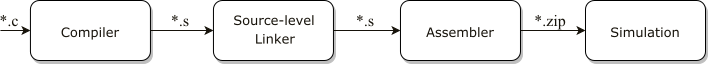
\includegraphics[width=.95\textwidth]{figures/linker_illustration1}
\caption{Workflow of simulation.}
\label{fig:linker_A}
\end{figure}

Doing the compilation and preprocessing steps from the compiler results in unlinked assembly code. Here symbols are not resolved yet, and it does not automatically generate a \emph{\_start} function. The source-level linker resolves the symbols and inserts a \emph{\_start} function in which the stack is initialized. However, the source-level linker works only for a single input file, therefore, all benchmarks are implemented in a single C file. The assembler and the simulator from the legacy toolchain are used and the source-level linker is necessary for the assembler to work. 

\begin{figure}[t]
\centering
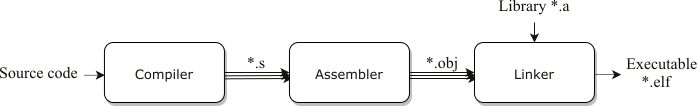
\includegraphics[width=.9\textwidth]{figures/linker_illustration2}
\caption{Standard linking process.}
\label{fig:linker_B}
\end{figure}

Figure \ref{fig:linker_B} illustrates the standard linking process when using the LLVM tools to do everything up to simulation. Other students have implemented an assembler and a linker within the LLVM framework. The assembler mainly consists of a parser that parses assembly code, and it uses LLVM-MC to form instructions to print them and the LLVM linker is developed within LLD. However, the new linker and assembler can not be used yet because it is still a work in progress.

%TODO: laat laatste 2 zinnen weg en voeg laatste zin uitgebreid toe



%Implementation of explicit datapaths using bypass registers.

%TODO: decide: comment or uncomment following section expl bp pass
%\subsection{Explicit Bypass Registers}
%This component implements the pass that we discuss in Section \ref{sec:expl_bp_impl} and thereby, implements the main goal of this project. It allocates explicit bypass registers on a machine function and it does that on a per basic block fashion using information of the pipeline state of other basic blocks. It uses \emph{BypassState} which keeps track of the bypass state of each basic block and can be configured to work on a given input state. This way the state of a pipeline can be analysed and remembered by the \emph{SimdExplicitRegister} pass after execution a basic block.

%\subsection{Instruction Printer}

%END COMPONENT DESCRIPTION

%\subsection{Assembler and Disassembler}



%Hier komt de uitleg v/d compiler implementatie en design. Bespreek hier eventuele tradeoffs die ik ben tegengekomen en design decisions die ik of anderen gemaakt hebben. Aangezien dit grotendeels een software project is, zou ik hier ook wat aandacht willen besteden aan software details, als in, bachelor software engineering skills erop los laten.  

%\Blindtext

\section{Exploiting Explicit Datapaths}\label{sec:expl_bp_impl}
This section describes the implementation and design decisions of the explicit datapath implementation on the LLVM-based compiler.

\subsection{Design Decisions}\label{sec:design_decisions}
%First, make the design space as large as possible
% tradeoffs/considerations/selection
% 1 or 2 solutions

First, let us list the design decisions. The first design decision is how to encode explicit datapaths such that the hardware knows about bypasses. Then there is the manner of when in the compilation chain does it actually encode these bypasses.
%TODO: extend with other decisions that are added below.

%TODO: add decision of how to encode the bypass registers. Choice to use register index space or add bits to instruction

%TODO: (is explained at class diagram 3.4.3) add decision for predicate flag instructions, we made getStartOperand to skip flagged instructions. Alternatively, it is also possible to ignore any flag operands that are encountered.

\subsubsection{Encoding bypasses}
The first design decision is how to encode that an operand is forwarded. There are two ways to encode that a source operand comes from the bypass network:
\begin{figure}[b!]
\centering
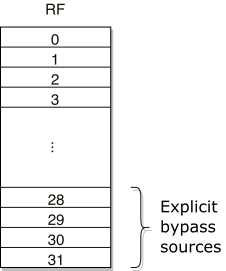
\includegraphics[width=.225\textwidth]{figures/encoding}
\caption{Illustration of reserving a portion of the register index space to encode explicit datapaths.}
\label{fig:rf_index_space}
\end{figure}

\begin{enumerate}[i.]
  \item Add bits to each instruction to specify that a certain operand comes from the bypass network. It requires three bits per source operands because there are five different bypass sources with a five-stage pipeline. Each instruction may have up to two source operands that can be bypassed. Therefore, this approach requires six additional bits to be added to each instruction.
  \item Use register index space to indicate that an operand comes from the bypass network. This requires at most five registers to be reserved because there are at most five bypass sources.
\end{enumerate} 

The approach in which the register index space is used to encode that an operand is bypassed was chosen because the hardware description of the architecture corresponds to that, and because this does not require any modification to the instruction format.

The other approach would be beneficial since it does not reduce the register file index space such that limitations to high register pressure can be avoided.

\begin{figure}[b!]
\centering
\subfloat[Explicit bypassing before RA.]{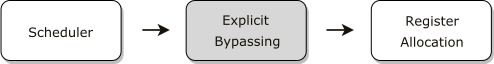
\includegraphics[width=.645\textwidth]{figures/explicit_bypass_allocationA}%
\label{fig:expl_bp_A}}
\vspace{10px}
\subfloat[Explicit bypassing after RA.]{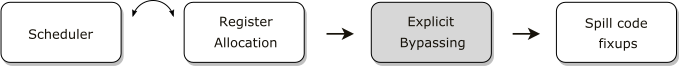
\includegraphics[width=.9\textwidth]{figures/explicit_bypass_allocationB}%
\label{fig:expl_bp_B}}
\caption{When to apply explicit bypasses.}
\label{fig:expl_bp}
\end{figure}

\subsubsection{When and how to allocate explicit bypasses}
When to actually do this can be categorized in three approaches. Trivially, it is not possible to do explicit bypass allocation before scheduling, because one needs a schedule to allocate explicit bypasses. %the order of instructions is not known at that time. 
(i) Ideally it would be done before register allocation (Figure \ref{fig:expl_bp_A}) where there are still virtual registers. The number of virtual registers reduces with each store that is avoided. Thereby, reducing register pressure and relaxing the job for the register allocator.

However, when the register allocator runs out of registers and inserts spill code between two instructions that were already bypassed, this bypass may not be valid anymore and may even require an additional register to undo that bypass.

(ii) Alternatively it can be done after register allocation. However, the physical registers that are freed by dead result elimination are not exploited when doing this after RA. Because, if spill code was necessary it has already been inserted during register allocation. Therefore, after the explicit bypasses have been allocated, the resulting assembly code may have redundant spill code and does not gain from reduced register pressure. With this approach it does not matter whether to do scheduling or RA first, which is illustrated in Figure \ref{fig:expl_bp_B}.

(iii) Finally, it is also possible to do scheduling and register allocation in one go with constraint programming. However, this problem is NP-complete and may take an unbounded amount of time. \\



%\begin{figure}[t]
%\centering
%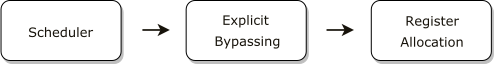
\includegraphics[width=.8\textwidth]{figures/explicit_bypass_allocation_A}
%\caption{Phase ordering problem.}
%\label{fig:expl_bp_A}
%\end{figure}

%\begin{figure}[b]
%\centering
%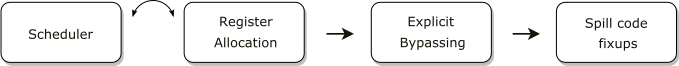
\includegraphics[width=.9\textwidth]{figures/explicit_bypass_allocation_B}
%\caption{Phase ordering problem.}
%\label{fig:expl_bp_B}
%\end{figure}

To summarize, ideally the explicit datapaths are exploited before register allocation to gain from reduced register pressure, but it is extremely difficult to insert spill code. So alternatively, it can be done after register allocation which may potentially have redundant spill code. For the later approach, an effort to clean up redundant spill code may be desired for more efficient code.\\

How to exploit explicit register allocation is a very broad question, in fact this is the main goal of this assignment. Let us split up in two categories of approaches:
\begin{enumerate}[i.]
  \item One way to exploit explicit datapaths is to group instructions close to their use. Moreover, if an instruction is strictly adjacent to its use, it may immediately be bypassed.%Group instructions together and allocate special bypass registers on the fly. Moreover, when this is done before register allocation where we have virtual registers, the number of virtual registers reduces with each bypass that we allocate. Thereby, reducing register pressure and relaxing the job for the register allocator.
  \item Another way to exploit explicit datapaths is by going through a basic block (a code sequence with no branches in except to the entry and no branches out except at the exit) and allocate explicit bypasses as a post-processing step, in the sense that this is done when the schedule does not change anymore.
\end{enumerate}

\begin{figure}[t]
\centering
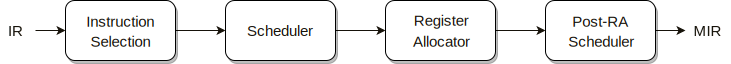
\includegraphics[width=.9\textwidth]{figures/phase_ordering}
\caption{Phase ordering problem.}
\label{fig:phase_ordering}
\end{figure}

The approach in the first category where instructions are grouped together has a problem. When a bypass is done early on, it needs to be verified if it is still valid after a change to the schedule has been made. In the compilation chain (Figure \ref{fig:phase_ordering}) the order in which instructions are executed is first decided by the general scheduler. The register allocator may insert spill code at any place in the schedule. After that, the order may change again by the post-RA scheduler or by a custom pass.\\

Now let us discuss the second approach that works on a basic block. The assumption in this approach is that the order in which instructions are executed is set and does not change anymore. Therefore, each bypass that is applied stays valid. 
%We can allocate explicit bypass register on an instruction if we have a RaW dependency between that instruction and an instruction in the pipeline state model.
The problem that remains is when there are multiple branches to the basic block. With multiple branches in, the state of the pipeline and which bypasses may be allocated can be different depending on which branch is taken. This problem is referred to as the join problem which is illustrated by example in Listing \ref{lst:join_problem}. Depending on which branch is taken the value of register \texttt{r7} may be forwarded from \texttt{ALU} when coming from \texttt{\%if}, or from \texttt{MUL} when coming from \texttt{\%else} which leads to an ambiguous pipeline state. Thus, the use of \texttt{r7} in \texttt{\%end} is forwarded from the bypass network, but is ambiguous and this together with being bypassed is not allowed for explicit datapaths. Therefore, such ambiguous behaviour should either be avoided or fixed, such that it is absent in the generated code.

\captionof{lstlisting}{Fragment of C code with corresponding assembly, to illustrate the join problem.}\label{lst:join_problem}
\begin{center}
\hspace{2px}\begin{minipage}{.475\textwidth}
\lstset{style=customc}
%\begin{lstlisting}[caption=List of instructions.,frame=tlrb]
\begin{lstlisting}[frame=tlrb]
int foo(int a, int b, int c)
{
  if (a > b)
    c += 5;
  else
    c = c * 3;
  c = c - a;
  return c;
}

<@\ @>
\end{lstlisting}
\end{minipage}\hfill
\begin{minipage}{.475\textwidth}
\lstset{style=customasm}
%\begin{lstlisting}[caption=IR-code.,frame=tlrb]
\begin{lstlisting}[frame=tlrb]
$foo:           # a = r5, b = r6 and c = r7
  sfles r5, r6
  bf    $else
  nop
$if:
  j     $end
  add   r7, r7, 5   # r7 in ALU
$else:
  mul   r7, r7, 3   # r7 in MUL 
$end:
  sub   r3, r7, r5  # r7 from MUL or ALU?
\end{lstlisting}
%\vspace{1.9em}
\end{minipage}
\end{center}

Bypassing with a limited scope of only a basic block requires multiple no-ops to be inserted on the end of each block, such that the pipeline state is flushed and no ambiguous behaviour occurs. Going from intra- to an inter basic block scope the ambiguous behaviour may be fixed using a technique which is discussed in the next section. With a function-level scope the pipeline state needs to be flushed only on a function call, because many instructions will be executed before returning. No-ops are not required because the prologue and epilogue insertions guarantee unambiguous behaviour between function calls. Going to a module-level scope would even allow bypasses from one function to another. However, because of time limitations, and because this only increases the bypasses with just a little bit, a module-level scope has not been implemented.\\

To conclude, the first approach discussed above may improve utilization of the bypass network, but can not be used as a stand-alone approach, since it does not solve the join problem. While the second approach works on a single basic block, it can easily be extended to a larger scope (for example, a function-level scope or a module-level scope). The following sections will show how the join problem can be tackled when a larger scope is considered. 

%When we bypass a value that is defined in another basic block, we require all blocks with a branch to that basic block to have that value in the same bypass source.

%REMOVE TEXT BELOW!!!
%We exploit explicit datapaths by going through a basic block (a code sequence with no branches in except to the entry and no branches out except at the exit) and allocate explicit bypass registers as a post-processing step, in the sense that we do this after scheduling, register allocation, packetizing, etc. Doing this as a post-processing step has advantages compared to doing this early on. 

%TODO: discuss add text below? ask Luc or Roel
%\begin{enumerate}[i.]
%\item When this is done after the packetizer it has bundled `VLIW' instructions consisting of both a scalar and a vector operation which reduces complexity of the bypassing approach.
%\item Another reason to do bypass allocation as a post-processing step is that doing it at an earlier stage, where the code is not certain yet, gives more problems. Each of the custom passes may reorder or insert instructions which may invalidate a bypass already allocated before that point.
%\end{enumerate}
%However, doing it early on also has an advantage.
%TODO: add problem with post-processing approach. Namely, doing this before register allocation reduces register pressure. RA tries to find a physical register for each virtual register. When we change some of these virtual registers with bypass registers already, we end do not need to find a physical register for these, thereby, reducing register pressure.

%clue


%TODO: continue writing xxx 


%This is where I will cover the software details and throw in some UML diagrams.
%\blindtext

\subsection{Join Problem}\label{sec:join_prob}
\begin{figure}[t!]
\centering
\subfloat[Fork-join in a loop.]{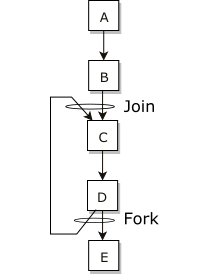
\includegraphics[width=.345\textwidth]{figures/cfg_fork_join_loop_widend}%
\label{fig:fork_join_loop}}
\hfil
\subfloat[Fork-join in an if-else statement.]{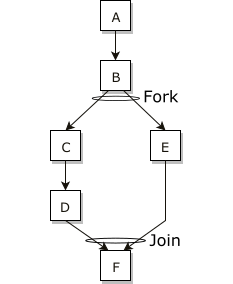
\includegraphics[width=.35\textwidth]{figures/cfg_fork_join_widend}%
\label{fig:fork_join_elif}}
\caption{Fork-join illustration in CFGs.}
\label{fig:fork_join_ill}
\end{figure}

The fork-join model typically branches off (fork) execution at a designated point in the program, and joins (merge) at a subsequent point to resume execution. %In parallel computing, this is a technique often used to spawn multiple processes that execute in parallel, which are at some point joined to sequential execution.
%TODO: if sentence above is added, add illustration of -<==>-
When a value is defined in between the fork and join points, and is forwarded to after the join point, it may be defined in one branch, but not or differently in the other branch/branches. When a bypass is encoded in an instruction, it is statically defined, in the sense that whatever branch is taken the value that is forwarded should always come from the bypass source that is encoded in the instruction. For example, take the following assembly code fragment, whatever path is taken to reach this point, the first source operand is always taken from the \texttt{ALU}, and the second source operand is taken from \texttt{MUL} unit.

\begin{lstlisting}
$join-point:
   add r1, ALU, MUL
\end{lstlisting}

Figure \ref{fig:fork_join_ill} shows two example CFGs with a join point. The following assembly code listings will illustrate how ambiguous bypasses may alter behaviour of the program. After that, a way to resolve such ambiguous behaviour is discussed.

\begin{lstlisting}
$A:
   <@$\vdots$@>
$B:
   nop             || v.addi r9,  r0,  32
   nop             || v.lw   r2,  r9,  0
   nop             || v.lw   r3,  r9,  1
   addi <@\hspace{1px}\textcolor{red!70!black}{r3}\hspace{1px}@>, r0, 16 || v.lw   r4,  r9,  2
   ori  r4, r0, 0  || v.addi r10, r0,  64
$C:
   lw   r6, <@\hspace{1px}\textcolor{red!70!black}{r3}\hspace{1px}@>, 3  || v.add  r12, CP,  r0
   lw   r6, <@\hspace{1px}\textcolor{red!70!black}{r3}\hspace{1px}@>, 2  || v.add  r13, CP,  r0
   lw   r6, <@\hspace{1px}\textcolor{red!70!black}{r3}\hspace{1px}@>, 1  || v.add  r14, CP,  r0
$D:
   nop             || v.mul  r12, r4,  r12
   nop             || v.mul  r13, r3,  r13
   addi r4, r4, 0  || v.add  r9,  CP,  r10
   addi r4, r4, 4  || v.add  r12, r12, r13
   sfne r4, 12     || v.mul  r14, r2,  r14
   bf   $C         || v.add  r14, r14, r12
   addi <@\hspace{1px}\textcolor{red!70!black}{r3}\hspace{1px}@>, r3, 32 || v.sw   r14, r9,  0
$E: <@$\vdots$@>
\end{lstlisting}

The assembly code fragment above for the CFG in Figure \ref{fig:fork_join_loop} shows a 3-by-3 matrix multiplication benchmark. In basic block \texttt{B}, each load operations loads a row from the vector memory. Then, each PE has an entire column stored in the RF. In each loop iteration (\texttt{CD}), one row of values is loaded from CP memory and communicated to the PE elements by basic block \texttt{C}. Subsequently, in block \texttt{D} each element of a row from scalar memory is multiplied with a value from a column. The results of the multiplications are added together, thereby, forming a row of the resulting matrix, which is then stored back to vector memory. 

When using the bypass network to forward a value from one basic block to another basic block, it is required that said value comes from the same bypass source regardless of the predecessor that is executed before it. For the matrix multiplication example, when bypassing the occurrences of \texttt{r3}, the value may be forwarded from \texttt{ALU} when predecessor \texttt{D} is executed, or from bypass source \texttt{WB} when predecessor \texttt{B} is executed. Note that this gives a conflict because \texttt{r3} does not come from the same bypass source in each of the predecessors. Therefore, a fix is required that puts the value in the desired bypass source. 

Considering that there can be any nummer of predecessors, the heuristic developed during this project takes the most frequently executed predecessor block as reference, and fixes all other predecessor to match. In this example, the loop body (\texttt{CD}) is executed more often than the loop header (\texttt{B}). Therefore, block \texttt{B} is modified such that it matches block \texttt{D}. To achieve this it can either swap the last two scalar operations in \texttt{B}. However, a more generic approach would be to insert an instruction at the end of \texttt{B} to put the value in the correct bypass source.

\begin{lstlisting}
$A:
   <@$\vdots$@>
$B:
   sfles r5, r6
   bf    $E
$C:
   <@$\vdots$@>
$D:
   j     $F
   addi  <@\hspace{1px}\textcolor{red!70!black}{r7}\hspace{1px}@>, r7, 5
$E:
   sub   r7, r7, r8
   mul   <@\hspace{1px}\textcolor{red!70!black}{r7}\hspace{1px}@>, r7, 3
$F:
   add   r3, <@\hspace{1px}\textcolor{red!70!black}{r7}\hspace{1px}@>, r5
\end{lstlisting}

The assembly code fragment above corresponds to the CFG in Figure \ref{fig:fork_join_elif}. It illustrates another example where a conflict may occur when forwarding a value over the join point to block \texttt{F}. In predecessor block \texttt{D}, the value in \texttt{r7} can be obtained by forwarding the result produced by the \texttt{ALU}. However, when predecessor block \texttt{E} is executed the value of \texttt{r7} may be forwarded from \texttt{MUL} instead. This conflict can be resolved by the same generic approach, namely, by inserting an operation at the end of either predecessor of \texttt{F} such that the value of \texttt{r7} may be forwarded using an identical bypass source, regardless of which predecessor is executed.


\subsection{Resolving Conflicts}\label{sec:conflicts}
When an operand can be bypassed, but has an ambiguous pipeline state, a simple correction is usually sufficient to make it unambiguous such that it can be bypassed. Ambiguous behaviour in the pipeline may occur when bypassing over a join point (a basic block that has multiple predecessors). The bypasses that are allocated when assuming the pipeline state of the most frequently executed predecessor is taken as reference, and when a different bypass would be allocated when assuming the pipeline state of another predecessor block, the other predecessor block is modified such that it matches the bypass allocation given by the reference block. Four cases are considered:

\begin{enumerate}
  \item If the reference forwards a value using \texttt{ALU}, but is not in \texttt{ALU} when another predecessor is executed. Then an operation is inserted to the end of these other predecessors which adds zero to the value that is bypassed.
  \item If the reference forwards a value using \texttt{MUL}, but is not in \texttt{MUL} when another predecessor is executed. Then an operation is inserted to the end of these other predecessors which multiplies the forwarded value with one.
  \item If the reference forwards a value using \texttt{LSU}, but comes from another bypass source by other predecessors. Then the load is copied, and inserted at the end of these other predecessors.
  \item When it is not possible to bypass the value from the reference block, but the other block or blocks do require a value to be bypassed. Then a nop is added to the end of the other predecessor(s) such that the value will be written back before it is used.
\end{enumerate}  

For a five-stage pipeline configuration an additional no-op is added when a multiplication or a load was inserted at the end of a block, so that the result is ready when it is used in the first operation of a basic block. This concludes all cases, however, the \texttt{WB} has not been considered. When the reference block forwards a value from \texttt{WB} over a join point, it requires an instruction to be inserted at a non-trivial position in the basic block, depending on where the uses occur. 


%TODO: add example where both a fix is needed, and a wb.

For this reason, the current implementation does not allow forwarding using \texttt{WB} over a join point. It achieves this by performing a check when the WB source is considered in a block that has multiple predecessors. It checks whether the instruction that defines the value and the instruction that it is forwarded to are in the same basic block, and whether the defining instruction dominates its use. If both conditions hold, then we are still good, since it is just being forwarded within a basic block and not over a join point.

This concludes the implementation of resolving ambiguous pipeline states. The next chapter is devoted to assessing the quality of the generated code by analyzing the simulation results.

%TODO: explain that we take the most-frequently executed predecessor block as reference, and fix all other preds to 'overeenkomen' met die block.

%OTOD: show with contradicting example that this approach doesnt work if also WB is considered. Therefore, it is not possible in the current implementation to bypass from the WB over a joint-point. 

%TODO: add scheduler/before RA/combined scheduling&RA/group instructions together to increase number of bypasses/ etc.
 
 
 
 %TODO: explain the difference between mandatory and non-mendatory bypasses (IN CHAPTER .3.4)

%\subsection{Class Diagrams}\label{sec:explicit_impl}
%%First, make the design space as large as possible
% tradeoffs/considerations/selection
% 1 or 2 solutions

%\begin{figure}[t!]
%\centering
%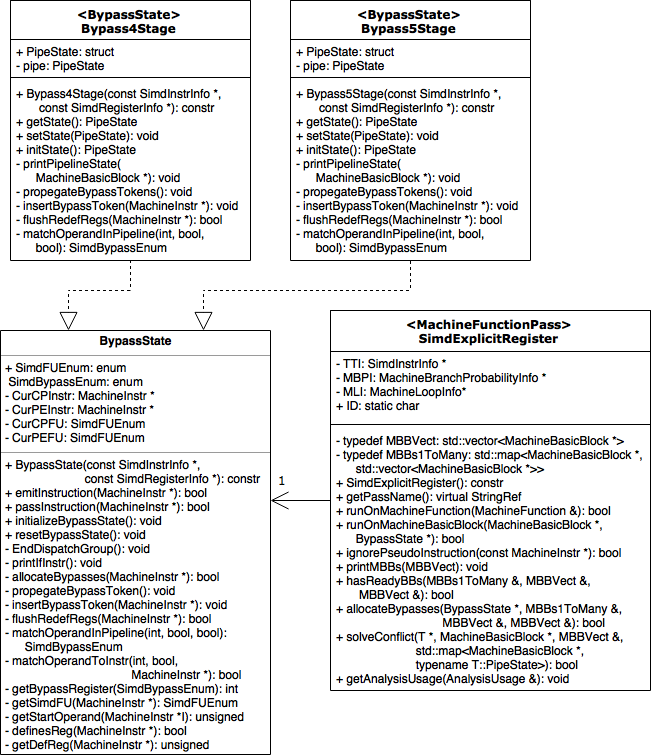
\includegraphics[width=.9\textwidth]{figures/class_diagram}
%\caption{Class diagram of the implemented approach to support explicit datapaths.}
%\label{fig:class_diagram}
%\end{figure}

There is a class called \texttt{BypassState} which should be inherited by each pipeline that we support, e.g. four-stage and five-stage pipeline. It models the values on busses in the bypass network. %It keeps track of values that reside in those busses which keeps track of the . We have This that can be 

\begin{figure}[b!]
\centering
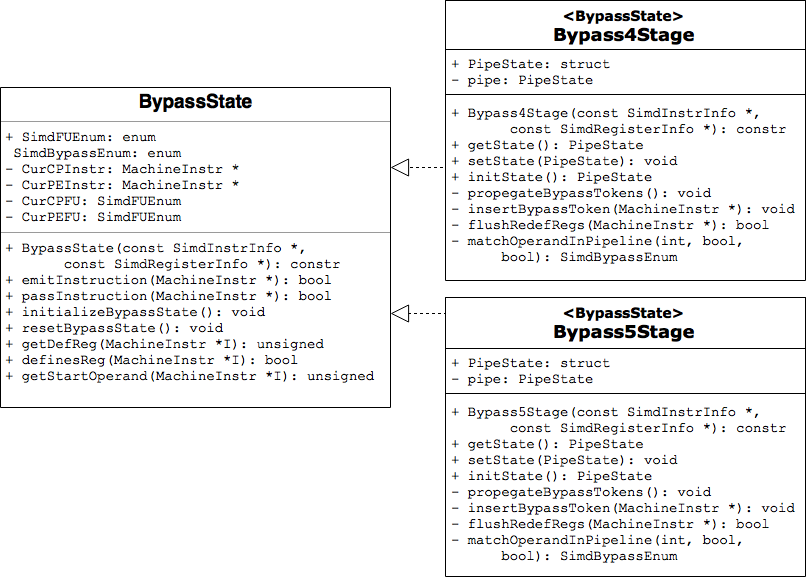
\includegraphics[width=\textwidth]{figures/class_diag_bpstate}
\caption{Class diagram for BypassState, and the inherited classes for the four-stage and five-stage pipelines.}
\label{fig:class_diagram_bpstate}
\end{figure}
%TODO: add following : there was a lot of functionality between the five stage pipeline and four-stage, so we define all shared functionality in \texttt{BypassState}, and stuff specific for a stage in \texttt{BypassXStage}.

We give a class diagram for \texttt{BypassState} in Figure \ref{fig:class_diagram_bpstate}. The classes  \texttt{Bypass4State} and \texttt{Bypass5State} represent the derived classes for the four-stage and five-stage pipeline respectively. Here we use \texttt{insertBypassToken} to pass the instructions in a basic block as tokens to \texttt{BypassState} one at a time and propagate the tokens each cycle using \texttt{propegateBypassTokens}. There is a variable in the derived classes, called \texttt{pipe} which represents the instructions that are currently in our pipeline. The pipeline state can be queried at any giving moment using function \texttt{getState}. This function can be used to acquire the state just before a jump or at the end of a basic block. The functions \texttt{initState} and \texttt{setState} may be used to initialize the state to a empty state, or a given state which is typically done at the beginning of a basic block. We use a function called \texttt{matchOperandInPipeline} to see what bypass can be allocated on a particular use operand of an instruction. It checks whether the operand uses a register defined by any of the instructions the pipeline (by calling \texttt{matchOperandToInstr} and \texttt{getDefReg} for each instruction can be forwarded). In general, it needs to find the newest definition of the register under consideration, therefore, when inserting a bypass token in the pipeline state we remove all occurrences using \texttt{flushRedefRegs}. This way we never have more than one instruction in the pipeline that define the same register, and thus always find the newest definition, if any.

Now lets continue with functions that handle instructions which are used to emit, pass or check an instruction (\texttt{emitInstruction}, \texttt{passInstruction} and \texttt{checkInstruction}). Emitting an instruction consists of the process of specifying which operations are in the current cycle and bypassing their operands according to the current pipeline state. Then pass instruction does the same, but the operands are not bypassed and check instruction does also not actually bypass the operands, but does keep the bypasses that it would allocate in a list. The functions \texttt{allocateBypasses} and \texttt{checkBypasses} do the actual bypassing work by calling \texttt{matchOperandInPipeline} which compares each operand of an instruction to  that can be bypassed. However, there are also flag operands that we do not consider. 
%\lstset{style=customasm}
%TODO: do something cool on the vector slots 
%\vspace{12px}
\begin{lstlisting}
    %loop
        sfgts r2, -64    || v.sfltu   P1, r1, 4
        bf    %loop      || v.slli.P1 r2, r1, 2
        add   r2, r2, -1 || v.add.P1  r7, r6, r2 
    %end:
                         <@\hspace{4px}$\vdots$@>
\end{lstlisting}

%TODO: move next paragraph to above listing, and remove newline
Flag operands occur before register source operands. The code fragment above shows an example of predicate instructions that uses flag operands to either do or not do a certain operation. In this case, we do a shift and add it with something if PE index is smaller than four ($P1$ is true). The function \texttt{getStartOperand} is used to skip flag operands. Alternatively we could also just ignore an operand if it is a flag operand. \\

After each cycle, a call is made to \texttt{EndDispatchGroup} which calls \texttt{insertBypassTokens} for each instruction in the current dispatch (can be two operations, a scalar and a vector op) and propagate the bypass tokens. So to summarize, operands are bypassed when they come across, and at the end of each cycle the pipeline is updated. %Meanwhile using getDef skip all instructions that occur but do not define an instruction. 


%TODO: verify and uncomment
%  later functions do not allocate bypass registers but may be used to insert instructions in the bypass state model, or to check which bypasses would be allocated according to a given bypass state (using \texttt{checkBypasses}), while the first one (\texttt{emitInstruction}) inserts the instruction into the bypass state model and allocates explicit bypasses wherever possible using \texttt{allocateBypasses}.


%TODO: verify and uncomment
% functions \texttt{getDefReg} and \texttt{definesReg} can be used to determine what is written to the register file by an operation, and \texttt{getStartOperand} may be used to see where in an operation we need to start with bypassing RaW dependencies. Function \texttt{matchOperandInPipeline} from the derived classes can be used to see if we can exploit one of the busses in a pipeline. We model these busses with a structure, called \texttt{PipeState}. 

%\begin{table}[b]
%\caption{Representation of struct PipeState.}
%\begin{center}
%\begin{tabular}{@{}l l@{}}
%\toprule
%\textbf{Type} & \textbf{Variable} \\
%MachineInstr* 	& Pipeline[N\_FUNCTION\_UNITS][N\_PACKET\_COUNT][EX\_STAGES]\\
%MachineInstr* 	& WB[N\_PACKET\_COUNT]\\
%SimdFUEnum	& issues[N\_PACKET\_COUNT][EX\_STAGES]\\
%{\small *: pointer}\\
%\bottomrule%%\\
%%{\small * pointer}
%\end{tabular}
%\end{center}
%\label{table:pipe_state}
%\end{table}%
